

\documentclass[12pt,a4paper]{report}
\usepackage[utf8]{inputenc}
\usepackage[T1]{fontenc}
\usepackage[british]{babel}

\usepackage{amsmath}
\usepackage{amsfonts}
\usepackage{amssymb}
\usepackage{makeidx}
\usepackage{graphicx}
\usepackage{float}
\usepackage[hidelinks]{hyperref}

\usepackage{listings}
\usepackage{color}
\usepackage{url}

\definecolor{dkgreen}{rgb}{0,0.6,0}
\definecolor{gray}{rgb}{0.5,0.5,0.5}
\definecolor{mauve}{rgb}{0.58,0,0.82}

\lstset{frame=tb,
  language=python,
  aboveskip=3mm,
  belowskip=3mm,
  showstringspaces=false,
  columns=flexible,
  basicstyle={\small\ttfamily},
  numbers=none,
  numberstyle=\tiny\color{gray},
  keywordstyle=\color{blue},
  commentstyle=\color{dkgreen},
  stringstyle=\color{mauve},
  breaklines=true,
  breakatwhitespace=true,
  tabsize=3
}



\title{Individual - Architecture Recovery}
\author{ (Nicklas Jeppesen) \\ Course code: KSSOARC2KU}
\date{May 10, 2024}



\begin{document}
	\maketitle
    \tableofcontents
    %\listoffigures

    
    
    \chapter{Introduction}
    The goal for this project is create a Static Analysis of the code base: https://github.com/zeeguu/API. 
    Where the goal should be to be able to take a given function and create a sequence diagram from the method.


    \section{Real work life motivation}
    Why this project? Why is this useful and why static analysis instead of dynamic analysis? 
    
    Motivation for this project, came by when I got a new job where I had to maintain an existing relatively large code base, where the code base was part of an eco-system of multiple systems, where the system could get a request from another system, and in the process of handling that request, performing other request to other systems, and to then return a response. There didn’t exists documentation that explain every single workflow, so to maintain and finding bugs became very hard. The idea was then, what if a system, could crossing systems, and create a sequence diagram, to visualize the dependencies of the other systems. Now micro-services and monolith distributed system has become more popular, so this idea might be useful for documentation existing code base in the future. 
    This project takes the first step on this journey and try to create a static analyzer which can analyze a single request method to create a sequence diagram from it, in the programming language python.

    \subsection*{Why static analyzer and not dynamic analyzer?}
    Its well known that static analyzer has several limitations that dynamic analyzer dont have, examples could be that, it can be difficult to determine dead code, whether it used or not, also if you have implemented the factory patterns in your code, it hard to say, if you have code that is never executed. So Dynamic analyzer seems to be a better option. Now in my real work case. I had two issues that speak against dynamic analyzer.

    first, I was not able to run the program local on my machine, because it needed specific installations files and licenses. Even then, we had servers where the system was installed, but then the second problem occur. It needed specific knowledge to trigger a given request in the system, from another system, that I didn’t have, so to trigger that request, I was forced to contact a colleague. These are the motivation for using a static analyzer, that can analyze not running code, to do reverse engineering to get an overview of the system. lastly, dynamic analyzer is easier in some language than others, like it easy in python, but more challenging in language like java, so implement static analyzer general can be easier, if someone need to do it, in another language.
    


    \chapter{Methodology}
    
    \section{Tools}
    First, this project used provided code from to colab pynb file. Thereafter it used the knowledge about dynamic and static analysis To actual analyse the non running code. Rich set of regex function was needed to be developed in the progress, for the following reason: 
    \begin{itemize}
        \item Used to extract the imported modules in a file, first inspired by the provided code, but later modified. 
        \item Regex is also used to get a list of all functions definiton in a file, used later to figure out which module/file a function call in a function is comming from. 
        \item Used to extract a function body from a file path, and a function name, to analyze. 
        \item Regex pattern matching is also used to get a list of function called in a function, for further analysis. 
    \end{itemize}
    
    \subsection{Creating the sequence diagram}
    For drawing the sequence diagram, I use a third party tool called 
     \href{https://github.com/mermaid-js/mermaid-cli}{mermaid-cli}, my code create a string that this tool can transform into a sequence diagram image file. 



    \chapter{Results}

    \section{What the code provide}
    By providing a filepath as string and function name to the function "analyze" in the file "zeep/static\_analysis\_ipynb", it output a png file naming the provided function name containing the the sequence diagram of function. The sequence diagram objects is the module names, that is because sometimes a file can import a function from a module and not a class, so a safe choice is to name the object the module name, and then horientizal line named name of the functions that are called. 
   
   
    \section{Workflow}
   
 
    \subsection*{How does the static analyzer work?}
    
    \paragraph{0: Master function:} The main function is named analyze, and can be find in the path: zeep/static\_analysis.ipynb, by scroling down. Its parameters is a function name as string, and a path to the file as string, and output a sequence diagram png file which has the name of the function. 

    \paragraph*{1: Get a list of module/functions calls:}
    by providing a file path and a function name the the analyze function, it first calls a function named GetfunctionsModuleUsedInfunction. 
    This return a list of module;function names, that the provided function is called that are defined in the code base, and not built in functions or from third party lib. 
    
    \paragraph{2: List into mermaid string:}
    After step 1, the analyze function take that list, and calls the function createMermaidString, which take this list, and transform it into a string, that mermaid-cli can read and understand. 

    \paragraph{3: From string into final sequence diagram:}
    Python has a built-in function, that allows the program to run terminal commands. Therefore when analyze function calls the function "generate\_sequence\_diagram", that take a mermaid-cli text string and the filename (function name) and run the mermaid-cli command, to create a sequence diagram file, the same location the code is running from. 
    
    \section{Output:}
    The final output of the, can be seem in the appendix figures. It contain sequence diagram for two of most used function sin the zeeguu-api project: 

    \begin{itemize}
        \item Function: "upload\_user\_activity\_data" from path: "zeeguu/api/endpoints/activity\_tracking.py"
        \item Function: "user\_articles\_recommended" from path: "zeeguu/api/endpoints/user\_articles.py"
    \end{itemize}



    


    \chapter{Discussion}

    \section{Challenges that I did not expect when starting}

    There was several surprises/challenges I faces, when started on this project. 

    \subsection{Filename not equal module name!}
    One challenge, I didnt expect, when I started this project, was that the imported module, might not be equal to the filename. 
    so to be able to extract a file path from its module name became very challenges, and I had the check the init.py file, to search for the correct name, and then again try to find the file name. 

    \section{General limitation of Static analysis}

    \section{Limitation for this codebase}
    To make this project not explored, I had to limit some kind of general code snippet, that python normal can accept which this static analyzer cannot, and these limitations are the following: 

    \subsection{Import from new line}
    The example below, shows an example, that my project cannot handle, because of the use of brackets and new line to import modules. This is one of the limitations I have to live with for now.

    \begin{lstlisting}
        #file: zeeguu/api/endpoints/activity_tracking.py
        from zeeguu.core.user_activity_hooks.article_interaction_hooks import (
            distill_article_interactions,
        )
        \end{lstlisting}

    To fix this issue, I change the code the the import module(s) is on a single line, which my code can handle. as shown below. 

        \begin{lstlisting}
            #file: zeeguu/api/endpoints/activity_tracking.py
             from <path> import distill_article_interactions
        \end{lstlisting}

    Another thing to note, The analyzer can handle multiple modules import from this, as just it is on one line. 
    
    \subsection{Import is not starting of the file}
    another issue I found, was if module is imported in the middle of the file, in a block, then the analyzer cannot register that, like the following issue: 
    \begin{lstlisting}
    #file: zeeguu/api/endpoints/activity_tracking.py, line 41
        if request.form.get("event") == "AUDIO_EXP":
            from zeeguu.core.emailer.zeeguu_mailer import ZeeguuMailer

            ZeeguuMailer.notify_audio_experiment(request.form, flask.g.user)
    \end{lstlisting}
    if the if statement becomes true, then this function call wont be registered, because the import module, was not registered. 
    i change this file too, so I added the from-import code in the top of the file, and then it was registered. 




    \section{Further development} 

    First thing is to correct the already found issues in the discussion section, this would be the first task. Second thing could be to expend this project, so it could have access to multiple code bases/microservices so it would be able to create sequences diagrams for a Kubernetes/docker swarm network. Third, to be able to create a deeper code analyzer, that either can analyze multiple code bases, or go deeper, into other methods call, one solution could be to create a tree structure, where the root node could be the first method and each sub node could be method calls in the methods, that calls methods either from the code base, or other code base we want to examinate, so we dont get system code into our tree. There from that tree, it could be possible to draw a sequence diagram, where each node could hold information about, codebase, module path, etc.. 


















    \chapter{Time allocation}

    Coding: 80\% \newline
    Writing report: 20\%


    \chapter{Github}

    \url{https://github.com/nicklasjeppesen/software_individual_report}
    
    \appendix
    \chapter{Appendix Figures}

    \begin{figure}[H]
        \centering
        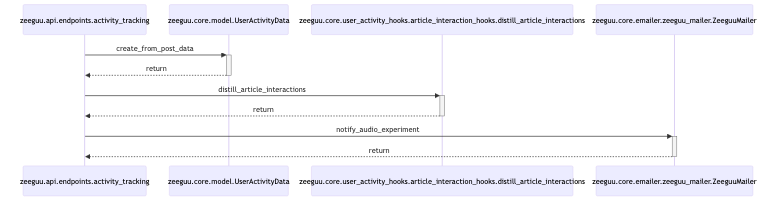
\includegraphics[scale=0.45]{upload_user_activity_data.png}
        \caption{Methods call for method \text{"upload\_user\_activity\_data"} in \text{"activity\_tracking.py"} }
        \label{upload_user_activity}
    \end{figure}
   
    \begin{figure}[H]
        \centering
        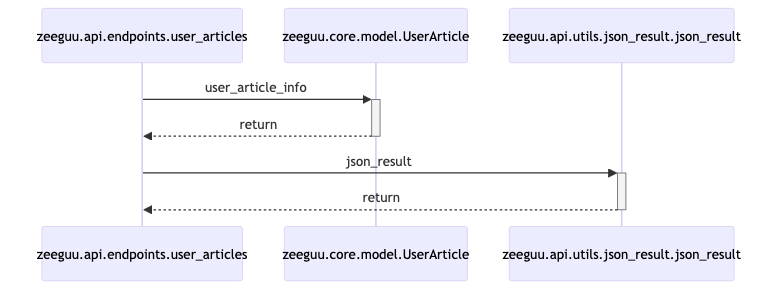
\includegraphics[scale=0.45]{user_articles_recommended.png}
        \caption{Methods call for method user\_articles\_recommended in file: user\_articles.py}
        \label{user_articles_recommended}
    \end{figure}
   





    \begin{thebibliography}{9}
        
        \bibitem{bl}Google colab code, url: \url{https://colab.research.google.com/drive/1oe_TV7936Zmmzbbgq8rzqFpxYPX7SQHP#scrollTo=0ruTtX88Tb-w}, (accessed: 09.05.2024).
        
        \bibitem{bl}Mermaid-cli: \url{https://github.com/mermaid-js/mermaid-cli}, (accessed: 09.05.2024).
       
        \bibitem{bl}reconstruction part 1: \url{https://github.com/mircealungu/reconstruction/blob/master/1_Introduction.md}, (accessed: 09.05.2024).
        \bibitem{bl}reconstruction part 4, dynamic analysis: \url{https://github.com/mircealungu/reconstruction/blob/master/4_Dynamic_Analysis.md}, (accessed: 09.05.2024).
       
        \bibitem{bl}Dynamic analysis, older material, but have other great examples of issues with static analysis: \url{https://github.com/mircealungu/reconstruction/blob/master/materials/Dynamic_Analysis.md}, (accessed: 09.05.2024).
       
    
    \end{thebibliography}
    

   
    
  
\end{document}


